\chapter{Introduzione}


\section{Motivazione}
Prova


\section{Gli attacchi DDoS}

Gli attacchi di Denial of Service (DoS) sono degli attacchi nel campo della sicurezza informatica che mirano a interrompere la fruizione di un servizio, fornito da un host connesso a internet, da parte di utenti legittimi. L'attacco ha l'obiettivo di esaurire le risorse dell'host in modo da non consentirgli di erogare le risposte ai richiedenti.
Nel caso in cui la sorgente del traffico che mira a creare disservizi non sia unica, si parla di attacchi di denial of service distribuiti (Distribuited Denial of Service).

\subsection{Tipologia di attacchi DDoS}
    
Gli attacchi DDoS possono essere suddivisi in due categorie principali in base al loro funzionamento. La prima si basa sul mandare alla vittima pacchetti malformati in grado di sfruttare un bug ana falla a livello applicativo. La seconda categoria invece si basa su tecniche per colpire l'infrastruttura del servizio, per il funzionamento di questa tecnica vengono usati uno o entrambi i seguenti metodi: uno punta sull'interruzione della connessione di rete grazie all'esaurimento della banda o della capacità di processamento dei router o di entrambe, nel secondo caso l'obiettivo dell'attaccante è di esaurire le risorse (es. sockets, CPU, memoria) del server che ospita il servizio \cite{ddos_survey_1}.

\begin{figure}[h]
    \label{1}
    % todo: capire come gestire citazioni immagini a livello di copyright
    %  e capire come funzionano le label per richiamar le immagini
    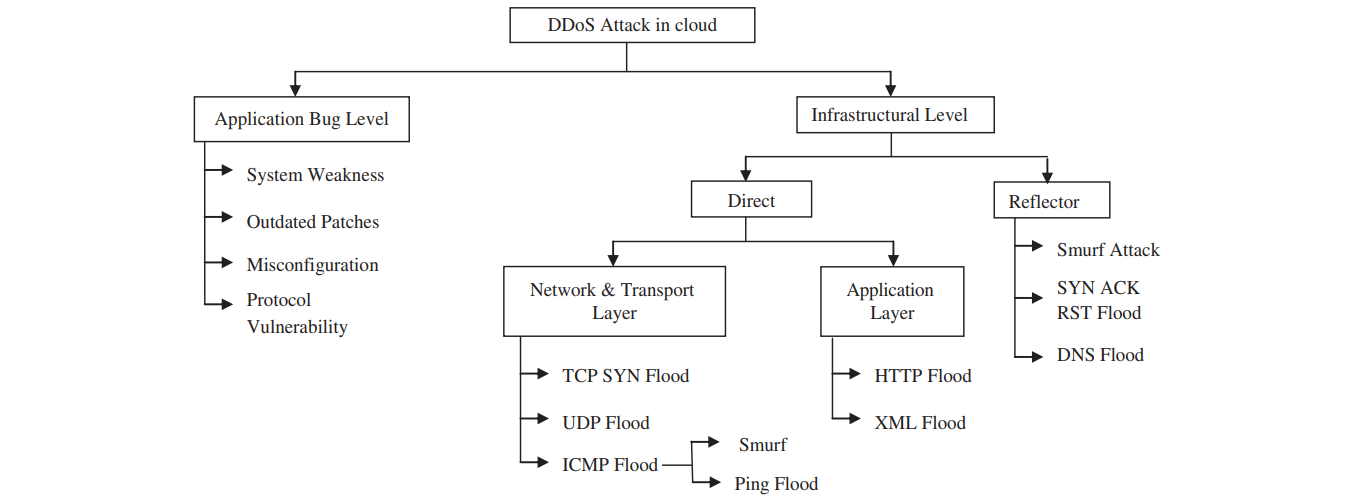
\includegraphics[width=\hsize]{images/introduzione/tipologie_ddos.png}
    \caption{Tipologie di attacchi DDoS}
    \centering
\end{figure}

L'obiettivo di questa sarà concentrato sul rilevamento e la mitigazione della seconda categoria di attacchi, basata sull'esaurimento delle risorse.

\subsubsection{Attacchi basati sul flooding}



\subsection{Vittime attacchi DDoS}
\subsection{Diffusione attacchi DDoS}


\section{Organizzazione della tesi}
